%----------------------------------------------------------------------------------------
%	PACKAGE SECTION
%----------------------------------------------------------------------------------------

\documentclass[12pt]{article}
\usepackage[utf8x]{inputenc}
\usepackage[english]{babel}
\usepackage{amsmath}
%\usepackage{hyperref}
\usepackage{graphicx}

\usepackage{pgfgantt,rotating}
\usepackage{epigraph}
\usepackage{xcolor, colortbl}

\usepackage{lastpage}
\usepackage{fancyhdr}
\pagestyle{fancy}

\renewcommand{\headrulewidth}{0.1pt}
\renewcommand{\footrulewidth}{0.1pt}
\fancyhead[C]{\textbf{Book Of Specifications}}
\fancyhead[R, L]{}
\fancyfoot[RO]{\textbf{\thepage/\pageref{LastPage}}} 
\fancyfoot[C]{PEnuts By CAPZ}

\begin{document}
%----------------------------------------------------------------------------------------
%	TITLE PAGE
%----------------------------------------------------------------------------------------
\begin{titlepage}
\newcommand{\HRule}{\rule{\linewidth}{0.4mm}} % Defines a new command for the horizontal lines, change thickness here

\center
\textsc{\Large Computer Project File}\\[0.1cm]
\textsc{\large SUP\---2022}\\[0.5cm]

\HRule \\
{ \huge \bfseries {PEnuts} \\
\LARGE Book Of Specifications \\[0.2cm]
\emph{\large{By CAPZ}}
}\\[0.2cm]
\HRule \\

\flushleft \Large \emph{}\\ 
  Alexandre POIRIER-COUTANSAIS\\
  Cloé LACOMBE\\
  Ziane LAYADI\\
  Pierrick MADE\\ 

\center {\large  version 1.0 \\ Friday, January 19, 2018}\\[0cm] 


\includegraphics[scale = 0.28]{Logo_EPITA.jpg}\\[1cm]

%\begin{figure}[h]
%\centering
%\begin{minipage}{.5\textwidth}
%  \centering
%  
\includegraphics[scale = 0.3]{Logo_EPITA}
%\end{minipage}%
%\begin{minipage}{.5\textwidth}
%  \centering
%  
\includegraphics[scale = 0.11]{Logo_EPITA}
%\end{minipage}
%\end{figure}


\end{titlepage}
\newpage

%----------------------------------------------------------------------------------------
%	Table of contents
%----------------------------------------------------------------------------------------

\pagenumbering{arabic}
\tableofcontents
\newpage

%----------------------------------------------------------------------------------------
%	DOCUMENT CONTENT
%----------------------------------------------------------------------------------------

\section*{Introduction} 

This year, as freshman students in Epita we have to do a six months computer project in groups of four. This project allows us to put into practice all knowledge acquired in lectures, tutorials and practicals but also to improve personal skills, which we have acquired for the chosen project, but which cannot be put into practice during course.\\

Our group is named CAPZ and we are working on a multi-player game. This game is PEnuts and his main concept is to evolve in a puzzle game with complementarity between players. The complementarity will mainly be based on different vision and possibles actions of each player. Indeed, even in a same room, players will not be able to see the same things or to interact with the same objects. As a puzzle game, the goal of our players will be to resolve enigmas to have access to next levels or rooms. This way, as they cannot evolve in solo, they will improve their ability to communicate and solve puzzle together.\\

The concept and ideas of the project do not come from a particular game. In fact, many aspects of the game already exist, but we did not want to be based on a specific game. We wanted to find a new game-play involving multi player cooperation and communication. Around this root, we developed the concept of complementarity and different visions of the environment. Which we finally chose to implement in a puzzle-game.\\

This book of specifications will present you in details the main points of our game project. In a first section it will give more information about the concept and origin of the project, containing videos games that inspired us or the objectives of the study. Then, in the second section there will be detailed organization of the work. In other words, there will be the distribution of the tasks, some details for each tasks and their estimated progression over time.\\

\newpage

%---------------------------------------------------------------------------
%	Type and Origin of Project
%---------------------------------------------------------------------------
\section{Type and origin of project}

	\subsection{The Concept of the project}
		As explained in the introduction, the main concept of our game is a complementarity and communication between two peoples to resolve a puzzle.
        \paragraph*{} To give a better view of what the game could look like, here is an example. In this example, we can see the vision of the level by each player.\\
        \paragraph*{} Here are the details to be able to understand the sketches of the next page.
        
		\begin{figure}[h]
		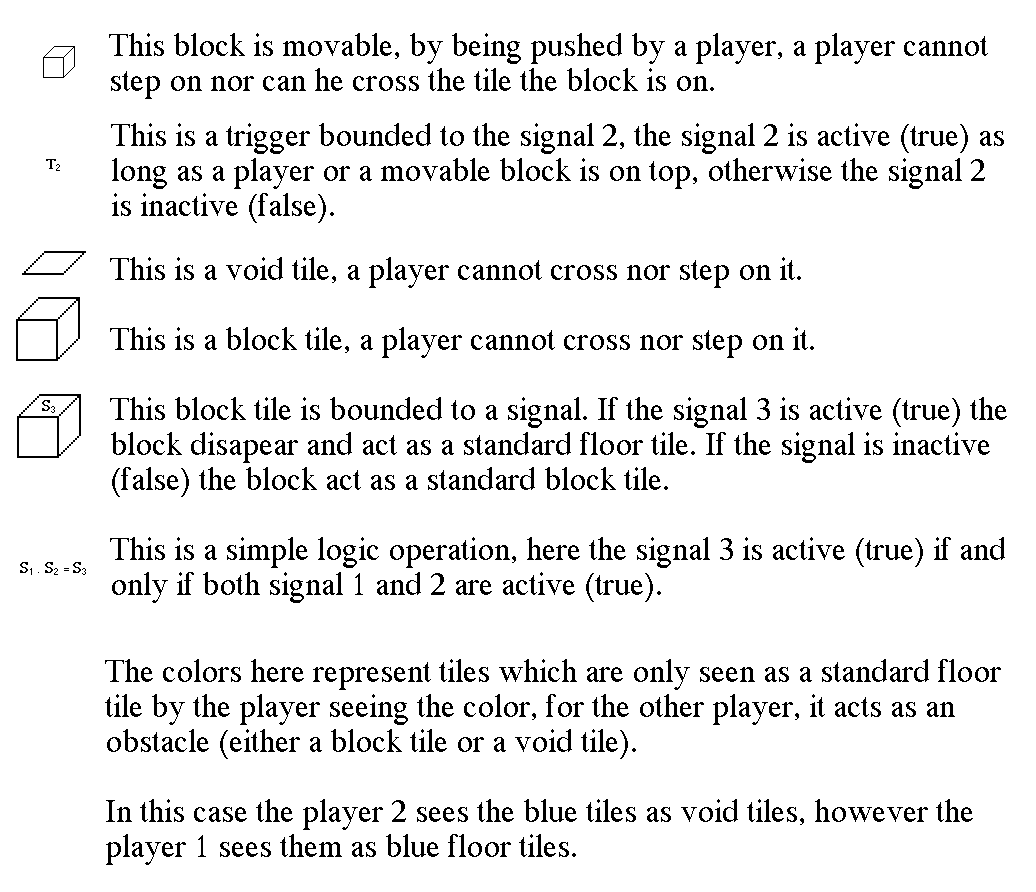
\includegraphics[scale = 0.5]{PEnuts_Concept_legend.png}
		\centering
		\end{figure}
		\begin{figure}[h]
		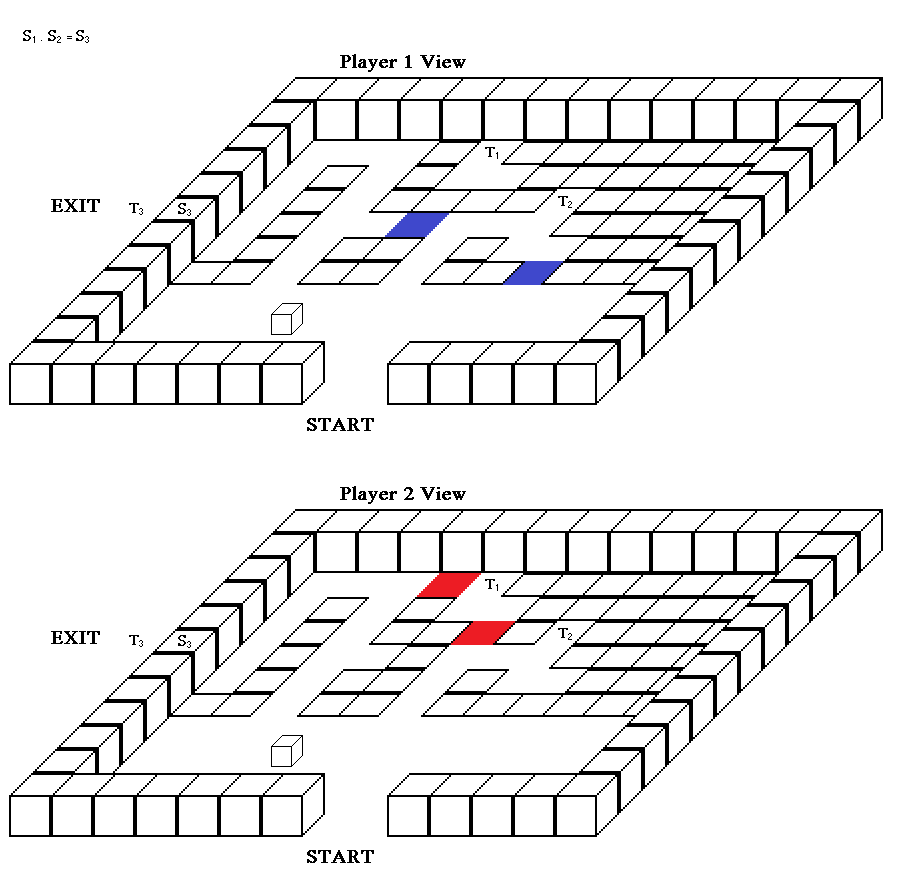
\includegraphics[scale = 0.55]{PEnuts_Concept_view.png}
		\centering
		\end{figure}
        
        In order to give a better idea of what will be our game, we decided to answer the main questions that can be asked for a Video Game.

		\subsubsection*{What is the main concept or specification of our game ?}
			We want to create a puzzle game mainly played in a cooperative way by two players. Then, the specification will be the complementarity between the different visions and actions of players.

		\subsubsection*{What is the goal of the players? How can they win ?}
			The Ultimate goal of the players is obviously to end the game by finishing all rooms. At lower scale, the goal of players is to finish a room to evolve in the game.\\
			But for us, a simple goal and the important goal of this game is the satisfaction to resolve a puzzle with a partner by communicating.
            
        \subsubsection*{How can they lose ?}
			There will be some objects able to kill players (a hole, a trap, an enemy). But as it is a puzzle game, players are "losing" if they do not manage to solve a room.

		\subsubsection*{In which environment players will evolve ? What will be the type of the map?}
			They will mainly evolve in rooms containing simple mechanism objects and obstacles. This will be a cubic environment with very simple details.

		\subsubsection*{What will be their possibles actions or movements ?}
			Players will be able to communicate with each other by using signal and voice. They will be allowed to interact with some objects. Finally, they are able to do simple movements, as walking.

	\subsection{Origin of the project}
		When we started talking about the project we tried to defined what each one of us wanted. In fact, what type of game do we want, what type of actions for the user, what type of environment, and so on.
        
 		\paragraph*{}Then, we pointed out that many games are good with only one physical characteristic changing (time, space, gravity, ...). They are easy to learn but hard to master. That was one of the specifications we wanted. Afterward, searching for a new original idea and concept to implement, we started on the idea of playing with the respective vision of the players. Finally, by developing our ideas and examples we ended up on this type of project.
		
        
	\subsection{Object of the study}
    	This project allow us to improve many of our skills. As a group or individually, it will give us many useful tools. This six months project will be for us one of our first real projects. Hence it will be completely rewarding for us.
        \paragraph*{}Here are the main skills that this project will give us :
        \begin{itemize}
        \item[-] Working as a group :
         	\begin{itemize}
                \item[-] Management
                \item[-] Team-working
                \item[-] Planning
                \item[-] Organization of a project
                \item[-] GitHub for a cooperative coding work
            \end{itemize}
        \item[-] Programming knowledge :
        	\begin{itemize}
            	\item[-] Network for multi player
                \item[-] Unity as our game engine
                \item[-] C\# for scripts in Unity
                \item[-] LaTex for documents and Reports
                \item[-] HTML/CSS for the website
                \item[-] Enhancing autonomous learning
            \end{itemize}
        \end{itemize}
         
         
    \subsection{State of the art}
    To think our game, we obviously had influence from all games we played in our lives, but some are more relevant, for example : \textit{Portal 2}, \textit{Zelda} and \textit{Keep talking and nobody explodes}\\
    
    
    The main aspect of \textit{Portal 2} is the same of our project, it is a puzzle-game. \textit{Portal 2} is really popular and is recognized as the best PC game of 2011 according to Metacritic. The player have to use his mind to cross different rooms using the 'portal gun' allowing him to create 2 portals in which he can travel. Here one aspect of the real world is changed and the player has to adapt and familiarize with this change. The cooperation mode allow for two players to cooperate to solve harder puzzles, requiring both player to use their portals to get through the rooms. The strength of the cooperation mode is that it combine both the puzzles and the social interaction between the players to create a unique game-play experience.\\

The \textit{Zelda} series is also a maze solving game where the player often has to complete different puzzles in Temples. This series is known by almost every gamer as one of the pillars of video-games. In this game the player has to combine different mechanics that he acquires through the game to solve puzzles and enigmas.
The player often need to think out of the box (in \textit{Zelda: phantom hourglass} on the Nintendo DS platform, the player, at one point, has to physically close the console in order to press a mold on his chart). It's strength relies on simple to difficult puzzles which forces the player to use his mind.\\

\textit{Keep talking and nobody explode} is a cooperation game where one player has to defuse a bomb while other players have to read a manual to give him instructions. This game is popular among many player groups as it always involve a strong cooperation between players. The manual in this game is really long and exhaustive and forces other players to read it and give instructions to the defuser since he can not in a reasonable time find every specification for each modules the bomb is composed of. Each module always has one and only one combination of actions that result in the deactivation of the module. The bomb is often composed of several modules which allow the defuser to give different task to different players, requiring coordination skills. It's main strength is the cooperation between the players coming from a simple game-play.\\

Those example are the most relevant examples compared to our project. We will therefore use the specified strengths of those game to improve our project.
\newpage

%---------------------------------------------------------------------------
%	Parts of the Project
%---------------------------------------------------------------------------
\section{Parts of the project}
To be able to keep a project organized and be able to respect deadlines, the tasks division can not be neglect. Therefore, this section will present in details the different tasks of our project, their distribution and their progression.\\[1.8cm]

\begin{table}[h!]
	\begin{center}
		\label{tab:table1}
		\begin{tabular}{|l||c|c|}
        	\hline
			& \textbf{Member} & \textbf{His}\\
			\textbf{Tasks} & \textbf{in charge} & \textbf{substitute} \\
			\hline \hline
			Player movements & \cellcolor{blue!25}Ziane & \cellcolor{red!25}Alexandre \\\hline
            Player Actions & \cellcolor{red!25}Alexandre & \cellcolor{blue!25}Ziane\\\hline
            Buttons/Mechanism & \cellcolor{red!25}Alexandre & \cellcolor{yellow!25}Pierrick\\\hline
			Camera and Lighting & \cellcolor{blue!25}Ziane & \cellcolor{yellow!25}Pierrick \\\hline
            Vision (what the player see)  & \cellcolor{blue!25}Ziane & \cellcolor{yellow!25}Pierrick\\\hline
            Collisions & \cellcolor{red!25}Alexandre & \cellcolor{green!25}Cloé\\\hline
            Color Codes & \cellcolor{yellow!25}Pierrick & \cellcolor{green!25}Cloé\\\hline
            Graphics & \cellcolor{green!25}Cloé & \cellcolor{blue!25}Ziane\\\hline
            3D Animations & \cellcolor{red!25}Alexandre & \cellcolor{yellow!25}Pierrick\\\hline
            Level Design & \cellcolor{green!25}Cloé & \cellcolor{pink!25}All\\\hline
            Sounds (effects) & \cellcolor{blue!25}Ziane & \cellcolor{yellow!25}Pierrick\\\hline
            Website & \cellcolor{yellow!25}Pierrick & \cellcolor{green!25}Cloé\\\hline
            Administration & \cellcolor{yellow!25}Pierrick & \cellcolor{green!25}Cloé \\\hline
      		Multi-player & \cellcolor{red!25}Alexandre & \cellcolor{green!25}Cloé\\\hline
            Network & \cellcolor{yellow!25}Pierrick & \cellcolor{red!25}Alexandre\\\hline
            Menu and Options & \cellcolor{green!25}Cloé & \cellcolor{yellow!25}Pierrick \\\hline
		\end{tabular}
		\caption{Task distribution}
	\end{center}
\end{table}


	\subsection{Programming}     
		\subsubsection{Players movements}
			In this part, the movements of the player will be implemented. Each player will be able to move in four directions and to jump.  
            
		\subsubsection{Players Actions}
			As it is a cooperation game, one of the main action that a player can do is to signal/point/ping something on the map. This will be useful to communicate with the other player.
            The player will also be allowed to interact with some objects. For example, he can push (or grab) a cube, he can also press a button.
            
        \subsubsection{Buttons \& Mechanism}
			This part can be seen as a subpart of the Level Design. It is in this section that we will configure and implement the different interactions of buttons (or switch) with the map.

		\subsubsection{Camera and Lighting}
			There will be two view for each player. Each player will have access to a third person view and a quick overview of the map.
     		The Lighting part is mainly for a most pleasant aspect.
            
        \subsubsection{Vision}
			Specific to our project, it will be the part where the differentiation between the two players in term of vision appears.
            
		\subsubsection{Collisions}
			Collisions are the interactions between the player and his environment (object, holes, and so on). In function of an object characteristics, the player will interact differently with it.

		\subsubsection{Level Design}
        	This part will be a major part of our project. It will be in this section that we will consider the creation of new type of puzzle, using mechanisms, visions and in fact the complementarity of the players.

		\subsubsection{Network}
			This section will be useful to handle the multi-player configuration. There will be some work to set the communication and data transfer between players.

		\subsubsection{Multi-player}
        	As we already implemented each player on their own, we will have to use network to put players together in the same game.
            
		\subsubsection{Menu \& Options}
        	In this part we will implement different options and interfaces to help and give some configurations to the user. Indeed, if the player can change the controls, add a joystick, mute the sounds effects, and so on, he will have a better experience of the game. 
	\newpage
	\subsection{Design}
        \subsubsection{Color Codes}
			We will need to do some choices to put good color codes in the game. Indeed, those colors will help players see something and will give informations. Those informations can be on the type of object, on the possible interactions, and so on. Hence this part can not be neglect to give a pleasant experience to players.
            
		\subsubsection{Graphics}
			The implementation of particles, polish assets and better appearance will be in this part. As the color codes, better the graphics appearance are better the comprehension and the experience of the player will be.
            
		\subsubsection{Sounds Effects}
        	This part, neglect in much projects, can in fact gives a real immersion to players. Hence, we will try to adapt sound effects and musics to the environment to give a more pleasant time.
    
   		\subsubsection{3D Animations}
			As the Graphics part, animations of players and fluidity of movements can only give a better aspect to the game and the environment.
    
    \newpage
    
    \subsection{Management}
		\subsubsection{Website}
			As the project will grow, we will have to do the same with a website. This website will contain :		 \begin{itemize}
        	\item[-] A project presentation
         		\begin{itemize}
                	\item[-] History
               		\item[-] Members
                	\item[-] Planning
                	\item[-] A Logbook (presenting for example the problems encountered)
            	\end{itemize}
        	\item[-] Links for downloads :
        		\begin{itemize}
            		\item[-] The Game
                	\item[-] Reports
                	\item[-] Other things used for the project (musics, pictures, videos,...)
            	\end{itemize}
        \end{itemize}           
		
        \subsubsection{Economic aspect}
        	This project is a nonprofit game. We will not earn any money on this creation. The aim of this project is mainly a contribution of knowledge.\\
            To finance this project we will not need money, except maybe for networks and severs.
		\subsubsection{Resources aspect}
        	For this project we will use mainly free and open-sources software as :
        		\begin{itemize}
            		\item[-] Unity (game engine)
                	\item[-] Overleaf (LaTex editor)
                	\item[-] MonoDevelop, Rider or VIM (C\# editor)
                    \item[-] Blender (3D animation and creation)
                    \item[-] CSS and HTML Editors
                    \item[-] GitHub (Coding organization)
            	\end{itemize}
\newpage


\subsection{Progression}

\begin{sideways}
\begin{ganttchart}[x unit=0.6cm, 
        y unit title=0.7cm,
        y unit chart=0.5cm,
        vgrid={*{8}{dashed}, red, dashed, dashed, dashed, dashed, dashed, red, dashed, dashed, red, red, red},
        vrule/.style={very thick, blue},
        hgrid, chart element start border=right]{1}{21}
\gantttitle{\textbf{Planning}}{21}\\
\gantttitle{January}{3}
\gantttitle{February}{4}
\gantttitle{March}{4}
\gantttitle{April}{4}
\gantttitle{May}{4}
\gantttitle{June}{2}\\

\ganttbar{Player movements}{1}{5} \\
\ganttbar{Collisions}{3}{8} \\
\ganttbar{Buttons/Mechanism}{2}{9} \\
\ganttbar{Vision}{2}{10} \\
\ganttbar{Multi-player}{4}{16} \\
\ganttbar{Network}{4}{13} \\
\ganttbar{Player Actions}{6}{10} \\
\ganttbar{Level Design}{6}{16} \\
\ganttbar{Color Codes}{6}{12} \\
\ganttbar{Camera and Lighting}{8}{10} \ganttbar{}{14}{16}\\
\ganttbar{Graphics}{13}{18}\\
\ganttbar{3D Animations}{14}{18} \\
\ganttbar{Sounds (effects)}{15}{17} \\
\ganttbar{Menu and Options}{13}{18} \\
\ganttbar{Presentations Preparation}{8}{9} \ganttbar{}{14}{15} \ganttbar{}{17}{19}\\
\ganttbar{Website / Project Reports}{7}{19} \\
\ganttbar{Administration}{9}{11} \ganttbar{}{15}{17} \ganttbar{}{18}{20}
\end{ganttchart}
\end{sideways}\\
To give an overview of the progression for each task, here is a Gantt Chart.

\newpage
\section*{Conclusion} %%see to disable number of this part...
This Book Of Specifications gave many informations about our project, PEnuts. We saw the main concept of the game : A Multi-player involving complementarity puzzle game. Then we saw its specification : players will have a different vision of the environment and different possible interactions. Furthermore, we saw the origin of the project, the object of the study, some examples of known games with similarities, the division and planning of the project, then some management aspects. All in all this book of specification is here to give a detailed vision of our project before its creation.\\[2cm]


\epigraph{`` Science isn't about WHY,\\it's about WHY NOT! ''}{\textit{ J.K. Simmons \\Portal 2}}

\end{document}
